\section{Introduction}


\begin{frame}
\frametitle{Introduction}
\framesubtitle{Contexte - 1}
%\tableofcontents


\begin{textblock*}{150pt}(43pt,105pt)
\footnotesize
Sant\'e
\end{textblock*}

\begin{textblock*}{150pt}(128pt,58pt)
\footnotesize
D\'efense
\end{textblock*}

\begin{textblock*}{150pt}(220pt,105pt)
\footnotesize
Industrie
\end{textblock*}

\begin{textblock*}{150pt}(190pt,205pt)
\footnotesize
Informatique
\end{textblock*}

\begin{textblock*}{150pt}(53pt,205pt)
\footnotesize
Economie
\end{textblock*}


\begin{textblock*}{50pt}(118pt,140pt)
\footnotesize\centering
\textbf{AMO Physics}\par
Recherche fondamentale
\end{textblock*}


\begin{textblock*}{200pt}(250pt,60pt)
\footnotesize
\begin{itemize}
\item La physique atomique d\'efinit le futur\footnote{\Tiny
N. R. C. Committee on AMO2010, Controlling the quantum world : the science of atoms,
molecules, and photons, ser. Physics 2010. National Academies Press, 2007}
\end{itemize}
\end{textblock*}


\begin{textblock*}{200pt}(250pt,100pt)
\scriptsize
\begin{itemize}
\item Quelques challenges \`a r\'esoudre pour les prochaines d\'ecennies
\end{itemize}
\begin{enumerate}
\item \scriptsize Opportunit\'es g\'en\'er\'ees par 
les avanc\'ees techniques dans le domaine des atomes froids 
\item \scriptsize D\'eveloppement de l'ing\'enieurie quantique et 
opportunit\'es \'economiques et sociales
\item \scriptsize Information quantique et potentielles 
applications dans les domaines de l'encryption et des cryptomonnaies
\item \scriptsize \textbf{Avanc\'ees promises par les 
nouvelles infrastructures \`a \'electrons libres et \`a rayons X (XFEL)}
\item \scriptsize \textbf{Promesses des impulsions laser ultra-br\`eves 
($\sim 10\,\rm fs$)
dans le contr\^ole ultra-pr\'ecis des atomes et mol\'ecules}
\end{enumerate}
\end{textblock*}

\begin{textblock*}{150pt}(50pt,65pt)
\scalebox{1}{
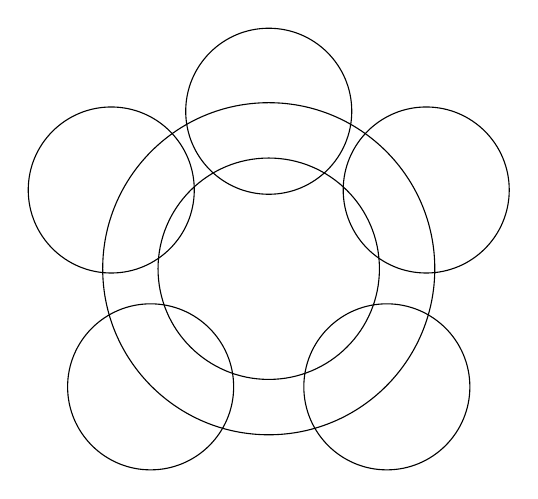
\begin{tikzpicture}
 %\node at (0,0) {};
%\fill (7,0) circle (2pt);
%\fill (6.30,0) circle (1pt);

%
%%\fill (6.5,1) circle (1pt);
%%\draw (6.30,0) to [bend left=45] (6.5,1);
%%\draw (6.5,1) to [bend left=45] (8,1.5);
%%\fill (8,1.5) circle (1pt);
  \draw (7,0) circle (40pt);
  \draw (7,0) circle (60pt);
  \draw (7,2) circle (30pt);
  \draw (9.,1.) circle (30pt);
  \draw (8.5,-1.5) circle (30pt);
  \draw (5.5,-1.5) circle (30pt);
  \draw (5.,1.) circle (30pt);
%\draw [->,thick,snake=snake] (5,3) -- (6.28,0.1);
%%\draw [->,snake=snake] (6.,3) -- (7.50,1.5);
%%\draw [->,snake=snake] (7.7,3) -- (8,2.5);
% \draw[solid,thick,->] plot [smooth] coordinates {(6.3,0)(7.5,2.2)(9.5,3.2)(10,3.4)};
% \node at (7.5,2.4){1};
% \node at (9.5,1.4){2};
% \draw[densely dashed,thick,->] plot [smooth] coordinates {(6.3,0)(7.5,1.5)(9.5,3)(7.3,.15)(10,1)};
%% \draw[densely dotted,thick,->] plot [smooth] coordinates {(6.3,0)(5.5,-1.5)(4.5,-2)(5.3,-.15)};
%% \draw[dotted,->] plot [] coordinates {(5.3,-.15)(6.3,0)};
%%\draw[] (6.3,0) to[out=100,in=100] (6.3,.1);
%%\draw[->] (6.30,0) to [bend left=45] (10,2.5);
%% \node at (7,.5) {\includegraphics[width=.7\linewidth]{../figures/chap3/sturm_mom_variation_nn_nbar.eps}};
\end{tikzpicture}
}
\end{textblock*}

\end{frame}


\begin{frame}
\frametitle{Introduction}
\framesubtitle{Contexte -2}
%\begin{itemize}
% \item Quelques grandes dates 
% \item Quelques grands faits
% \item Int\'er\^et et applications
%\end{itemize}

\begin{textblock*}{250pt}(20pt,60pt)
\includegraphics[scale=.35]{../figures/chap2/pulse_length_evol.eps}\\
\includegraphics[scale=.35]{../figures/chap2/theoretical_intensity.eps}\\
\end{textblock*}


\begin{textblock*}{250pt}(200pt,70pt)
\footnotesize
\begin{itemize}
 \item La situation
\begin{itemize}
\scriptsize
\item Grandes avanc\'ees exp\'erimentales 
\item Grandes avanc\'ees en informatiques
\item Manque de mod\`eles th\'eoriques adapt\'es
\end{itemize}
\end{itemize}
\end{textblock*}

\begin{textblock*}{250pt}(200pt,120pt)
\scriptsize
\begin{itemize}
\item L'espace des configurations (EC) et ses limites pour la description 
de l'ionisation 
\begin{itemize}
\scriptsize
\item Non-localit\'e de la fonction d'onde
\item Difficult\'es analytiques
\item Co\^ut num\'erique tr\`es important
 \item Inadaptation de l'EC
pour la description de l'ionisation
%en champ intense et de haute intensit\'e 
\end{itemize}
\scriptsize
\item Solutions possibles
\begin{itemize}
\scriptsize
\item Techniques de gestion des reflexions aux bornes
\item Utilisation d'une jauge diff\'erente
\item Utilisation de l'approximation du champ fort
\item \textbf{Utilisation de l'espace des moments}
\end{itemize}

\end{itemize}
\end{textblock*}

\end{frame}


\begin{frame}
\frametitle{Introduction}
\framesubtitle{Motivation}

\begin{textblock*}{250pt}(10pt,70pt)
\includegraphics[scale=.33]{../figures/chap2/dip_app_limits.eps}
\end{textblock*}

\begin{textblock*}{250pt}(200pt,60pt)
\scriptsize
\begin{itemize}
 \item Fait: Sup\'eriorit\'e de l'espace des moments sur 
l'espace des configurations pour la description de l'ionisation
 \item Probl\`eme: Co\^ut num\'erique venant avec le avantages physiques 
\end{itemize}

\end{textblock*}


\begin{textblock*}{250pt}(200pt,120pt)
\begin{itemize}
\scriptsize
\item N\'ecessit\'e de d\'epasser l'approximation du champ fort 
(\acrshort{sfa}) et de r\'eint\'egrer le potentiel coulombien 
dans la dynamique de l'interaction rayonnement-mati\`ere dans l'\acrshort{em}
\item N\'ecessit\'e d'une formulation analytique \textbf{simple}
et efficace du potentiel coulombien non local
\item N\'ecessit\'e d'une technique de r\'esolution 
num\'erique de l'\'equation de Schr\"odinger viable du points de 
vue des performances et des ressources informatiques
\item \textbf{Besoin d'un mod\`ele de r\'esolution num\'erique 
performant en temps de calcul sans compromission des r\'esultats}
%\item \textbf{Mise au point d'un mod\`ele permettant d'envisager 
%la r\'esolution de l'\'equation de Schr\"odinger au del\`a de 
%l'approximation dipolaire}
\end{itemize}

\end{textblock*}

\end{frame}



%\begin{frame}
%\frametitle{Introduction}
%\framesubtitle{Plan}
%\tableofcontents
%\end{frame}
